\documentclass[conference]{IEEEtran}
\IEEEoverridecommandlockouts
% The preceding line is only needed to identify funding in the first footnote. If that is unneeded, please comment it out.
\usepackage{cite}
\usepackage{titlesec}
\usepackage{amsmath,amssymb,amsfonts}
\usepackage{algorithmic}
\usepackage{graphicx}
\usepackage{textcomp}
\usepackage{xcolor}
\def\BibTeX{{\rm B\kern-.05em{\sc i\kern-.025em b}\kern-.08em
    T\kern-.1667em\lower.7ex\hbox{E}\kern-.125emX}}
\begin{document}

\title { \HUGE {Kocaeli Üniversitesi}\\
\LARGE {Bilgisayar Mühendisliği Bölümü}\\
\huge \textbf{Programlama Laboratuvarı 1}\\
\huge{Proje 2}}

\author
{
\IEEEauthorblockN{\large Robera Tadesse GOBOSHO}
\IEEEauthorblockA{\large ID:190201141\\
\textit{\large robtad318@gmail.com}}


\and
\IEEEauthorblockN{\large Muhammad Abdan SYAKURA}
\IEEEauthorblockA{\large ID:200201147\\
\textit{\large prof.syakur@gmail.com }}
}


\maketitle
\section*{\textbf{\LARGE Özet}}
\Large{ Bu projenin amacı sonek ağaçlarını ve sonek katarlilerini kullanarak katarlar üzerinde bazı arama
işlemleri yapmaktır.
Bir katar için sonek, katarın herhangi bir karakterinden başlayarak sonuna kadar olan kısımdır.
Sonek ağaçları doğal olarak asimetriktir: önek uzantıları yalnızca birkaç güncellemeye neden olurken, sonek uzantıları tüm son ekleri etkiler ve bir güncelleme dalgasına neden olur. Sonek ağacının kenarlarını, örtük düğümlerin aynı davranışı sergilediği, bantlarin verilen benzer kenarların koleksiyonlarına ayırdık ve örtük düğümlerin bantlar içinde "yüzmesine" izin vermek için açık uçlu kenarlar kavramını kullandık. İç örtük düğümler, açık ek ağaç düğümleri ile birbirinden ayrılır. Bu özellikler, örtük düğüm güncellemelerinin dalgalarını takip etmek ve son ek ağacını amortize edilmiş cizgi olarak oluşturmak için kullanıldi.\\
Bu proje kapsamında sonek ağaçları kullanılarak s katarı için sonek ağacı oluşturulabilir, Sonek ağacı oluşturulan bir s katarı içinde p katarı geçip gecmedigi kontrol edilecek, geçiyorsa ilk bulunduğu yerin
başlangıç pozisyonu ve kaç kez tekrarlandığı görüntülenecektir,Sonek ağacı oluşturulan bir s katarı içinde tekrar eden en uzun altkatar bulunacak ve ekrana kaç kez tekrarlandığı yazılacak, Sonek ağacı oluşturulan bir s katarı içinde en çok tekrar eden altkatar bulunup, kaç kez tekrarlandığı ekrana yazilacak.
}


\section*{\textbf{\LARGE G\.{ı}R\.{ı}Ş}}
Bir rn-karakter katarı S için bir ağaç Τ son eki, 1'den m'ye kadar numaralandırılmış tam olarak m yaprağı olan köklü, yönlendirilmiş bir ağaçtır. Kök dışındaki her bir dahili düğümün en az iki çocuğu vardır ve her kenar boş olmayan bir S alt katarı ile etiketlenir. Bir düğümün hiçbir iki kenarı aynı karakterle başlayan kenar etiketlerine sahip olamaz. Sonek ağacının temel özelliği, herhangi bir yaprak I için,
kökten I yaprağına giden yoldaki kenar etiketlerinin sıralanması, i konumunda başlayan S son ekini tam olarak heceler. Yani S[i..m]'yi heceliyor. Örneğin, xabxac katarı için son ek ağacı Şekil:1'de gösterilmiştir. Kökten I numaralı yaprağa giden yol tam dava S = xabsac'ı, 5 numaralı yaprağa giden yol ise ac son ekini heceler. S'nin 5. konumunda başlar.Yukarıda belirtildiği gibi, S için bir sonek ağacının tanımı, herhangi bir katar için bir sonek ağacının gerçekten var olduğunu garanti etmez.


\begin{figure}[h]
    \centering
    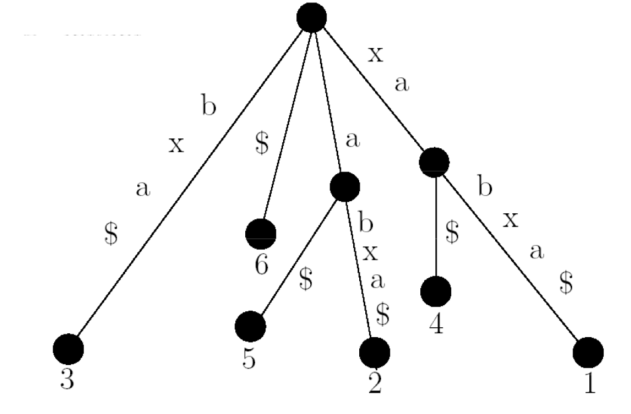
\includegraphics[scale=0.5]{suffix tree fig.png}
    \caption{xabxa katarı için sonek ağacı}
    \label{Şekil:1}
\end{figure}



\section*{\textbf{\LARGE Yöntem}}

\subsection{\textbf{\Large Tanım}}\label{SCM}
Dize için sonek ağacı S uzunluk nşöyle bir ağaç olarak tanımlanır: 

\begin{itemize}
\item Ağacın numaralandırılmış tam olarak n yaprağı vardır 1 için n.

\item Kök dışında, her dahili düğümün en az iki çocuğu vardır.

\item Her kenar, boş olmayan bir alt dize ile etiketlenir. S.

\item Bir düğümden başlayan hiçbir iki kenar, aynı karakterle başlayan dize etiketlerine sahip olamaz.

\item Kökten yaprağa giden yolda bulunan tüm dize etiketlerini birleştirerek elde edilen dize i son eki heceler S[i..n],için i itibaren 1 için n.

\end{itemize}
Tüm dizeler için böyle bir ağaç bulunmadığından, Sdizede görülmeyen bir uçbirim simgesiyle doldurulur (genellikle \$.)\\

Örnek olarak şekil 2'yi alırsak, "BANANA" kelimesinin sonek ağacı. Her alt dize özel karakter \$ ile sonlandırılır. Kökten yapraklara giden altı yol (kutular olarak gösterilir) altı son eke karşılık gelir A\$, NA\$, ANA\$, NANA\$, ANANA\$ ve BANANA\$. Yapraklardaki sayılar, ilgili son ekin başlangıç konumunu verir. Kesik çizgilerle çizilmiş son ek bağlantıları inşaat sırasında kullanılır.

\begin{figure}[h]
    \centering
    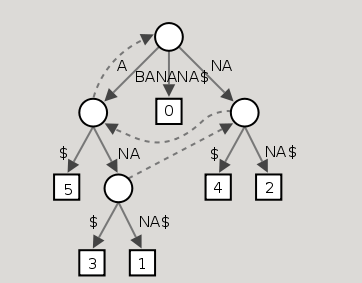
\includegraphics[scale=0.75]{banana suffix tree diagram.png}
    \caption{"BANANA" katarı için sonek ağacı diyagramı}
    \label{Şekil:2}
\end{figure}


\subsection{\textbf{\Large Örtülü sonek ağacı oluşturma}}\label{AA}
bu projede, sonuncusu S katarınin gerçek bir sonek ağacına dönüştürülen bir katar örtülü sonek ağacı kullanıldı.
S katarı için bir örtülü sonek ağacı, S\$ için sonek ağacından, \$ terminal sembolünün her kopyasını ağacın kenar etiketlerinden kaldırarak, ardından etiketi olmayan herhangi bir kenarı kaldırarak ve ardından en az iki çocuğu olmayan herhangi bir düğümün kaldırarak elde edilen bir ağaçtır. S'nin S[l..i] öneki için örtülü bir sonek ağacı, S[1..i]\$ için sonek ağacı alınarak ve yukarıda açıklandığı gibi \$ sembollerini, kenarları ve düğümleri silerek benzer şekilde tanımlanır. S[1..i] katarınin örtülü sonek ağacını I i için 1'den m'ye kadar gösteriyoruz. Herhangi bir S katarı için örtülü sonek ağacı, yalnızca S'nin son eklerinden en az birinin başka bir sonekin öneki olması durumunda, S\$ katarı için sonek ağacından daha az yaprağa sahip olacaktır.\\

\begin{figure}[h]
    \centering
    \includegraphics[scale=0.5]{Suffix tree for string xabxa.png}
    \caption{xabxa\$ katarı  için sonek ağaç diyagramı}
    \label{Şekil:3}
\end{figure}

\begin{figure}[h]
    \centering
    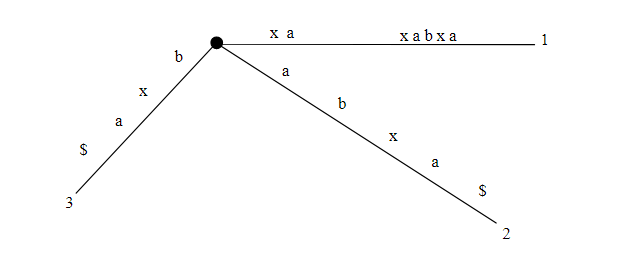
\includegraphics[scale=0.5]{Implicit suffix tree for string xabxa.png}
    \caption{xabxa\$ katarı  için örtülü sonek ağaç diyagramı}
    \label{Şekil:4}
\end{figure}

Bu durumdan kaçınmak için tam olarak S'nin sonuna terminal sembolü \$ eklendi. Bununla birlikte, S, S'de başka hiçbir yerde görünmeyen bir karakterle biterse, o zaman S'nin örtülü sonek ağacının her sonek için bir yaprağı olacaktır ve bu nedenle gerçek bir sonek ağacı olacaktır. Örnek olarak, Şekil 3'te gösterilen xabxa\$ sting için xa soneki, xabxa son ekinin bir önekidir ve benzer şekilde a dizgisi de abxa'nın bir önekidir. Bu nedenle, xabxa için sonek ağacında, 4 ve 5 numaralı yapraklara giden kenarlar yalnızca \$ ile etiketlenir. Bu kenarların kaldırılması, her biri yalnızca bir çocuklu iki düğüm oluşturur ve daha sonra bunlar da kaldırılır. xabxa için elde edilen örtük son ek ağacı Şekil 4'te gösterilmektedir. Bir örtülü sonek ağacının her bir sonek için bir yaprağı olmasa da, S'nin tüm soneklerini kodlar. Her sonek, örtülü sonek ağacının kökünden gelen bir yoldaki karakterler tarafından hecelenir. Ancak yol bir yaprakta bitmiyorsa yolun sonunu gösteren bir işaret olmayacaktır. Bu nedenle, örtülü sonek ağaçları, kendi başlarına, gerçek sonek ağaçlarından biraz daha az bilgilendiricidir. örtülü sonek ağacını S için gerçek sonek ağacını elde etmek için Ukkonen'in algoritmasında bir araç olarak kullandık.\\\\


\section*{\textbf{\LARGE YALANCIKOD (PSEUDOCODES)}}

\begin{figure}[h]
    \centering
    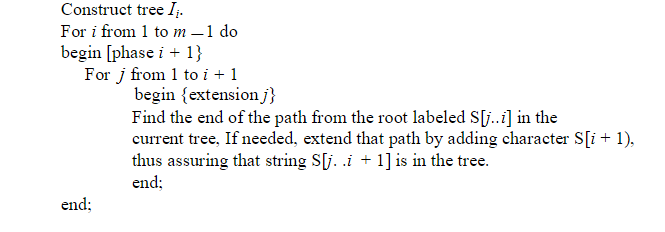
\includegraphics[scale=0.6]{generalPseudocode.png}
\end{figure}
\begin{figure}[h]
    \centering
    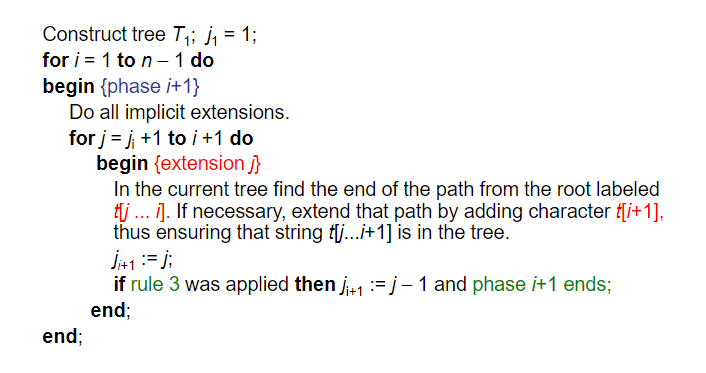
\includegraphics[scale=0.5]{extended pseudocode for Ukk.png}
    \caption{Ukk için genişletilmiş yalancıkod}
\end{figure}

\begin{figure}[h]
    \centering
    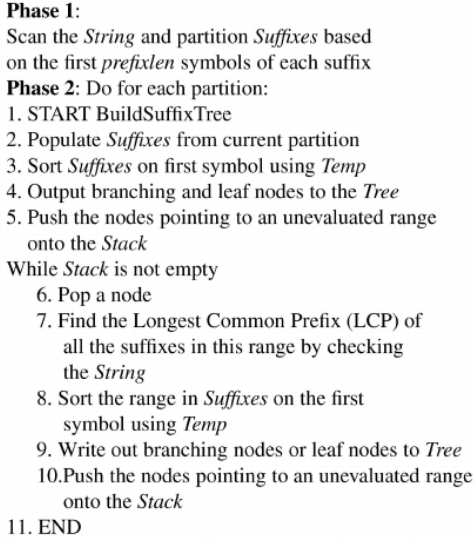
\includegraphics[scale=0.7]{PWOTD.png}
    \caption{ Partition and Write Only TopDown}
    
\end{figure}




.\\\\\\\\\\\\\\\\\

\section*{\textbf{\LARGE Deneysel Sonuçlar}}

Program iki girdi alır: a) sonek ağacının oluşturulacağı katar ve b) girilen katarnin altkatarı. Kullanıcının girdileri girmesinin iki farklı yolu vardır. İlk yöntem, programın kendisinde aranacak dize ve alt dizeyi girmektir. İkinci yol, çalışma zamanı sırasında katarnin bulunduğu dosyanın adını ve altkatarı  main fonkisyon parametresi olarak girmektir. Aşağıda şekil 7 ve şekil 8'de gösterildiği gibi, her ikisinin de çıktısı tamamen aynıdır.\\
Girdileri aldıktan sonra program aşağıdaki çıktıları verir:
\begin{itemize}
\item S katarı için bir sonek ağacı oluşturur.
\item S sonek ağacının p altkatarın içerip içermediğini kontrol eder. içeriyorsa, altkatarın bulunduğu ilk pozisyonu gösterir ve altkatarın kac kere tekrar ettigini görüntüler.
\item Sonek ağacı oluşturulan bir s katarı içinde tekrar eden en uzun altkatar bulur ve kaç kez tekrar ettigini gosterir.
\item Sonek ağacı oluşturulan bir s katarı içinde en çok tekrar eden altkatarı bulur ve kaç kez tekrar
ettigini goruntuler.
\end{itemize}
\begin{figure}[h]
    \centering
    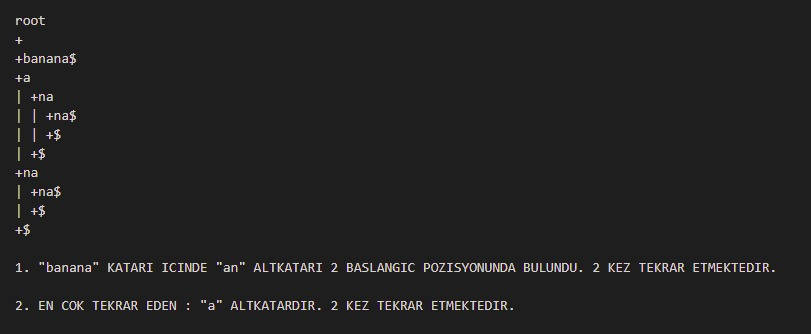
\includegraphics[scale=0.3]{output1.jpg}
    \caption{}
\end{figure}

\begin{figure}[h]
    \centering
    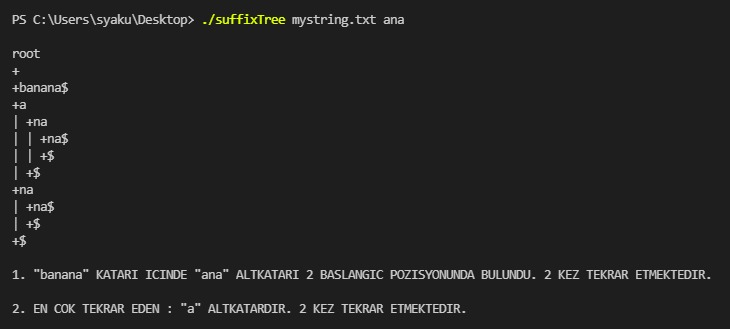
\includegraphics[scale=0.3]{output2.jpg}
    \caption{}
\end{figure}

\newpage

\section*{\LARGE Kaynakça}
\begin{thebibliography}{00}
\normalsize
\bibitem{b1} https://core.ac.uk/reader/82138620

\bibitem{b2} Algorithms on Strings, Trees, and SequencesDan GusfieldUniversity of California, DavisCambridge University\\ Press1997
\bibitem{b3} https://tr.hrvwiki.net/wiki/Suffix\_tree.

\bibitem{b4}  http://web.stanford.edu/~mjkay/gusfield.pdf
\bibitem{b5} http://fragglet.github.io/c-algorithms/

\bibitem{b6} http://www.vilo.com/edu/2002-03/Software/Loeng5\\\_Suffix\_Trees/Suffix\_Trees
\\/cs.haifa.ac.il/shlomo/suffix\_tree/


\bibitem{7} https://www.youtube.com/watch?v=3CbFFVHQrk4
\bibitem{8} https://www.youtube.com/watch?v=N70NPX6xgsA
\bibitem{9} https://visualgo.net/en/suffixtree
\bibitem{10} https://www.tutorialspoint.com/cprogramming/c\_\\command\_line\_arguments.htm
\bibitem{11} https://rosettacode.org/wiki/Suffix\_tree
\bibitem{12} https://stackoverflow.com/questions/737257/how-to-convert-c-code-to-c
\bibitem{13} https://www.geeksforgeeks.org/enumeration-enum-c/
\bibitem{14} https://www.youtube.com/watch?v=qh2leThTv0Y

\bibitem{15} Book Algorithms on Strings, Trees and Sequences: Computer Science and Computational Biology by Dan Gusfield
\bibitem{16} https://developerinsider.co/graphics-graphics-h-c-programming/
\bibitem{17} https://www.geeksforgeeks.org/represent-tree-using-graphics-in-c-c/
\bibitem{18} https://www.sanfoundry.com/cpp-program-implement-suffix-tree/
\bibitem{19} https://en.wikipedia.org/wiki/Longest\_repeate\\d\_substring\_problem
\bibitem{20} https://dmcconnell-comp150.herokuapp.com/suffix\\\_trees/construction
\bibitem{21} https://stackoverflow.com/questions/3306279/tries-and-suffix-trees-
implementation
\bibitem{22} https://stringfixer.com/tr/Suffix\_tree
\bibitem{23} https://caetanogenete.github.io/Visualise-Suffix-Tree/
\bibitem{24} https://www.overleaf.com/

\end{thebibliography}


\end{document}
